\hypertarget{results}{%
\section{5. Results}\label{results}}

\hypertarget{learning-over-the-declared-horizon}{%
\subsection{5.1. Learning over the declared
horizon}\label{learning-over-the-declared-horizon}}

\begin{minipage}{\linewidth}

\emph{Full validation at call 10,000; two model-initialization seeds,
fixed data order.}

\begin{center}
\begin{tabular}{@{}
  >{\raggedright\arraybackslash}p{(\columnwidth - 8\tabcolsep) * \real{0.1579}}
  >{\raggedleft\arraybackslash}p{(\columnwidth - 8\tabcolsep) * \real{0.2105}}
  >{\raggedleft\arraybackslash}p{(\columnwidth - 8\tabcolsep) * \real{0.2105}}
  >{\raggedleft\arraybackslash}p{(\columnwidth - 8\tabcolsep) * \real{0.2105}}
  >{\raggedleft\arraybackslash}p{(\columnwidth - 8\tabcolsep) * \real{0.2105}}@{}}
\toprule\noalign{}
\begin{minipage}[b]{\linewidth}\raggedright
Seed
\end{minipage} & \begin{minipage}[b]{\linewidth}\raggedleft
Stock QR10 CE
\end{minipage} & \begin{minipage}[b]{\linewidth}\raggedleft
Full BF16 CE
\end{minipage} & \begin{minipage}[b]{\linewidth}\raggedleft
CE increase
\end{minipage} & \begin{minipage}[b]{\linewidth}\raggedleft
Perplexity increase
\end{minipage} \\
\midrule\noalign{}
204 & 3.411152 & 3.422389 & +0.011237 & +1.130\% \\
205 & 3.409272 & 3.419354 & +0.010082 & +1.013\% \\
\bottomrule
\end{tabular}
\end{center}

\end{minipage}

The mean paired endpoint increase is \textbf{0.010659815 CE}. Both seeds
show a larger early gap: at call 500, BF16 exceeds the reference by
0.123913 and 0.118438 CE for seeds 204 and 205. From call 2000 onward
the observed gaps remain approximately 0.007--0.012 CE, rather than
continuing toward zero. The pilot's FP32-state warm arm already shows a
comparable call-500 gap (0.118346 CE); all four warm-policy pilot arms
span 0.118--0.125 CE there. Thus the early deviation is not specific to
BF16 storage. QR20 roughly halves it on this prefix, consistent with a
refresh-policy contribution. The pilot does not causally separate
cadence, tracking, arithmetic and storage effects at the final horizon.
This behavior supports reporting the full curves rather than only
endpoint agreement. Two initialization seeds with fixed data order
provide limited replication; we make no statistical equivalence claim or
confidence-interval interpretation.

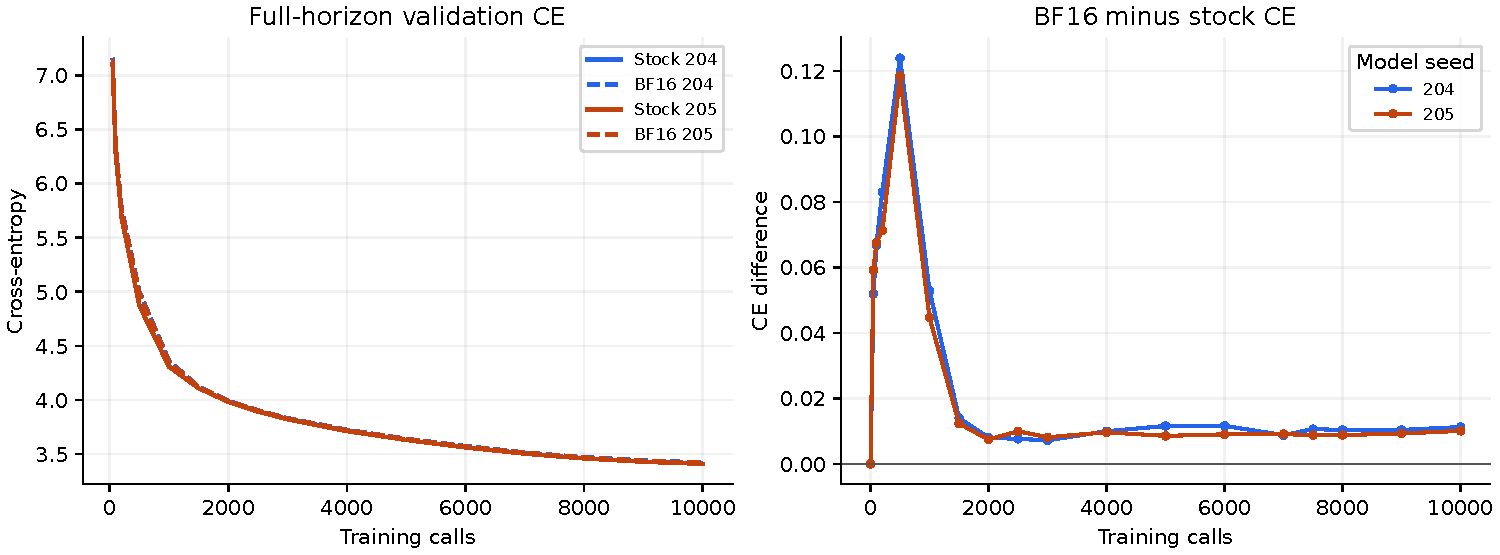
\includegraphics{figures/full_horizon.pdf}

\emph{Figure 1.} Left: the declared learning horizon, displaying
observations from call 50 onward. Right: BF16 minus stock CE, including
the shared initial value. Lines connect observed evaluations; they do
not represent additional measurements.

\hypertarget{time-and-memory}{%
\subsection{5.2. Time and memory}\label{time-and-memory}}

\begin{minipage}{\linewidth}

\emph{Synchronized steady-step wall means; evaluation, diagnostics and
startup excluded.}

\begin{center}
\begin{tabular}{@{}lrrrr@{}}
\toprule\noalign{}
Seed & Matched calls & Stock step ms & BF16 step ms & Time reduction \\
\midrule\noalign{}
204 & 101--200 & 380.740 & 314.638 & 17.36\% \\
205 & 101--10000 & 380.548 & 309.533 & 18.66\% \\
\bottomrule
\end{tabular}
\end{center}

\end{minipage}

Seed 205's timing includes 9,900 calls, covering 198 complete 50-call
cycles. Seed 204's newly paired timing includes only calls 101--200 on
the replay device; its cached full reference is used for quality, not
relabeled as newly paired timing. These different windows should not be
averaged into one speed estimate. The short seed-204 window is within LR
warmup but covers two complete 50-call event cycles. Sequential arms
share a claimed device; GPU clocks and thermal state were not controlled
or logged.

Persistent matrix state falls from 2,491,416,576 to 1,245,708,320 bytes
(2.320 to 1.160 GiB; approximately 50\%). Seed 205's peak allocated
tensor memory falls from 9.397 to 8.223 GiB. Peak allocation includes
diagnostic allocations and is distinct from device reservation or
persistent state alone. That is approximately 12.49\% lower peak
allocation, compared with the approximately 50\% matrix-state reduction.
The BF16 state total includes 32 bytes for four groups' FP32 age/LR
scalars.

Complete-step means include forward/backward, matrix packing and writes,
and auxiliary AdamW. Diagnostic and evaluation work is outside the timed
step scopes and inside campaign elapsed accounting. Compiler caches are
shared sequentially within campaigns. The step means do not estimate
first-use compilation cost or whole-run time-to-quality, and the
combined implementation comparison does not isolate warm tracking as the
cause of all time savings. Each forward/backward and optimizer interval
is measured with synchronized host wall time, with GPU synchronization
at phase boundaries. This prevents overlap across those boundaries; its
effect relative to an asynchronous training loop, including any unequal
effect on eager and compiled execution, was not isolated.

Seed 205's recorded optimizer means can be accounted for by event class.
Mean optimizer time falls from 95.23 to 26.08 ms/call, a 3.65-fold
ratio. Ordinary events cost 34.44 ms in stock versus 10.14 ms in the
candidate; QR events cost 642.37 versus 601.18 ms, and candidate warm
events cost 61.61 ms. The shared timing window contains 90\% ordinary
events in both arms; stock has 10\% QR events, while the candidate has
8\% warm and 2\% QR events. Consequently 47.28 of the 69.15 ms/call
optimizer saving (68.38\%) lies in refresh events, and 21.87 ms/call
(31.62\%) in ordinary events. The whole-step difference is 71.02
ms/call. This identity is descriptive accounting of observed means, not
a causal separation of cadence, batching, compilation, arithmetic, and
storage. In particular, both refresh frequency and per-event execution
differ.

\hypertarget{short-sparse-qr-controls}{%
\subsection{5.3. Short sparse-QR
controls}\label{short-sparse-qr-controls}}

\begin{minipage}{\linewidth}

\emph{Seed 204; full 10k LR horizon; timing calls 101--2000. Original
FP32 stock and cached warm timing come from separate launches; this is
mixed-implementation context.}

\begin{center}
\begin{tabular}{@{}lrrrr@{}}
\toprule\noalign{}
Policy & CE at 500 & CE at 2000 & Step ms & Optimizer ms \\
\midrule\noalign{}
Stock QR10 (pilot) & 4.877601 & 3.985905 & 382.773 & 96.358 \\
Warm10/QR50 (cached) & 5.001514 & 3.993939 & 314.142 & 26.415 \\
QR20 & 4.936852 & 3.990383 & 329.641 & 40.460 \\
QR50 & 5.018046 & 3.998679 & 313.551 & 22.864 \\
\bottomrule
\end{tabular}
\end{center}

\end{minipage}

These two fresh controls use the same full-BF16 arithmetic, coverage,
efficient QR primitive, seed 204, data, and full 10,000-call
learning-rate horizon. QR20 sets both refresh and repair periods to 20;
QR50 sets both to 50, producing no warm events. The warm comparison
reuses the first 2,000 calls of the completed main candidate. Complete
shared timing cycles span calls 101--2000. The stock row is the original
FP32-state reference's pilot prefix; it is not a matched full-BF16 QR10
control.

At call 2000, warm is 0.003557 CE behind QR20 and 0.004740 ahead of
QR50. Warm has lower CE than QR50 at all seven noninitial validation
observations; QR20 has lower CE than warm at six. These repeated panels
are not independent seeds. The warm prefix has extra refresh work for a
modest quality gain over holding bases between QR50s. Its timing comes
from the earlier launch, so the small whole-step difference from QR50 is
contextual rather than a fresh paired timing result. On this prefix QR20
reaches lower CE at about 4.93\% greater measured step time than cached
warm. The timing comparison spans launches and supplies no calibrated
noise interval. The study establishes neither QR20 superiority over warm
at the full horizon nor the converse; both orderings remain open.

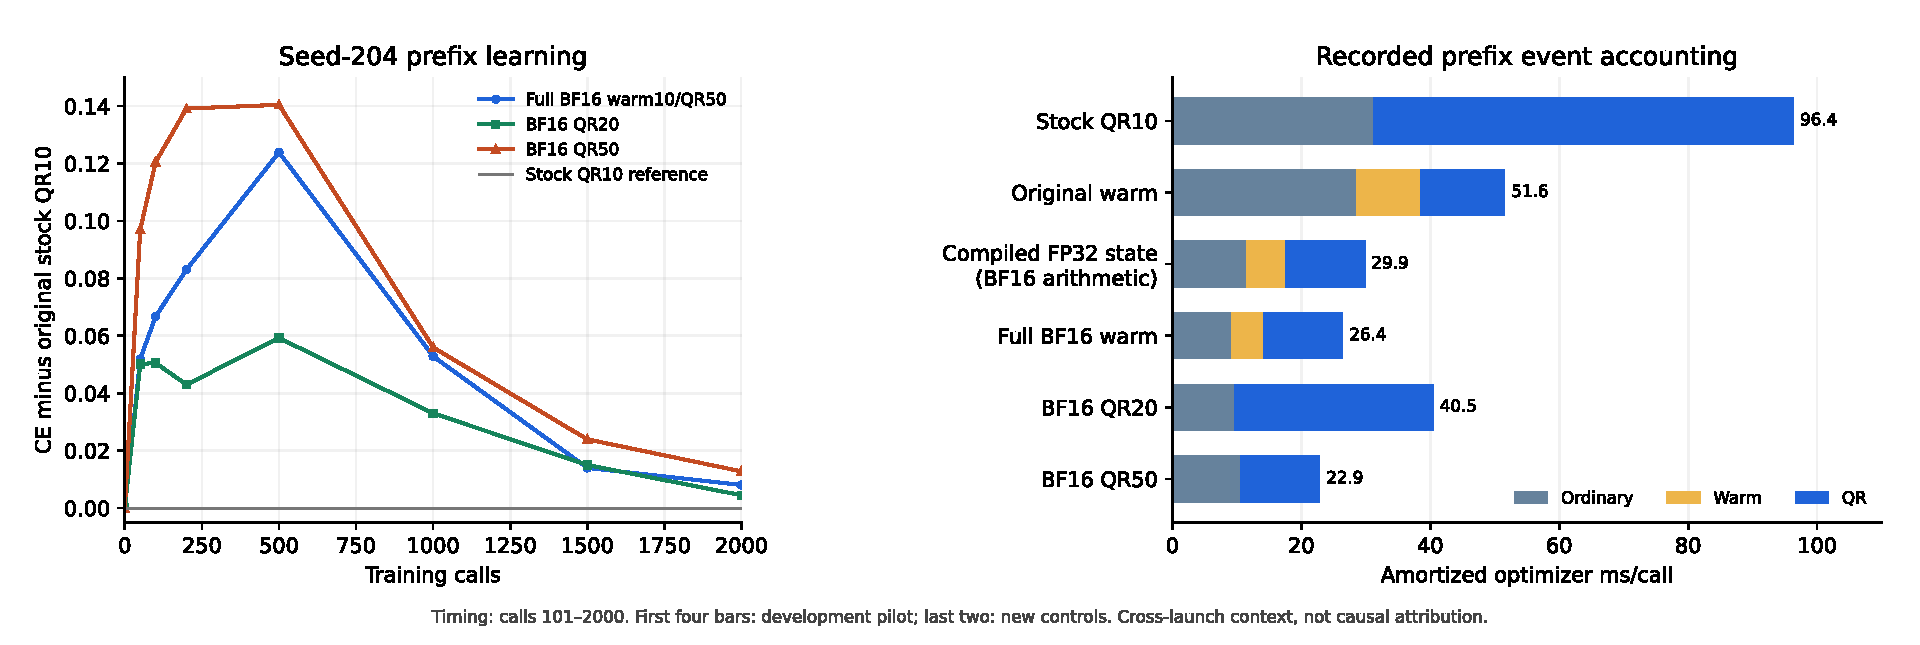
\includegraphics{figures/review_tradeoff.pdf}

\emph{Figure 2.} Left: seed204 CE relative to the original stock QR10
prefix. Right: optimizer event-class means weighted by their frequencies
over calls 101--2000. The first four bars use the development pilot;
QR20/QR50 use the new controls. Original/compiled warm policies use
warm10/QR50. The bars describe mixed-implementation, cross-launch
context and are not causal ablations.

\hypertarget{what-qr-product-reuse-explains}{%
\subsection{5.4. What QR product reuse
explains}\label{what-qr-product-reuse-explains}}

\begin{minipage}{\linewidth}

\emph{Synthetic matched-input QR primitive; CUDA-event medians, batch
12.}

\begin{center}
\begin{tabular}{@{}
  >{\raggedright\arraybackslash}p{(\columnwidth - 8\tabcolsep) * \real{0.1579}}
  >{\raggedleft\arraybackslash}p{(\columnwidth - 8\tabcolsep) * \real{0.2105}}
  >{\raggedleft\arraybackslash}p{(\columnwidth - 8\tabcolsep) * \real{0.2105}}
  >{\raggedleft\arraybackslash}p{(\columnwidth - 8\tabcolsep) * \real{0.2105}}
  >{\raggedleft\arraybackslash}p{(\columnwidth - 8\tabcolsep) * \real{0.2105}}@{}}
\toprule\noalign{}
\begin{minipage}[b]{\linewidth}\raggedright
Dimension (batch 12)
\end{minipage} & \begin{minipage}[b]{\linewidth}\raggedleft
Original CUDA ms
\end{minipage} & \begin{minipage}[b]{\linewidth}\raggedleft
Reuse CUDA ms
\end{minipage} & \begin{minipage}[b]{\linewidth}\raggedleft
Time reduction
\end{minipage} & \begin{minipage}[b]{\linewidth}\raggedleft
Reordered columns
\end{minipage} \\
\midrule\noalign{}
768 & 31.210 & 30.914 & 0.95\% & 0/9216 \\
1536 & 82.053 & 80.535 & 1.85\% & 12/18432 \\
2304 & 145.854 & 141.566 & 2.94\% & 40/27648 \\
3072 & 225.660 & 215.218 & 4.63\% & 160/36864 \\
\bottomrule
\end{tabular}
\end{center}

\end{minipage}

The profile uses identical fixed synthetic C/Q inputs within each pair,
BF16-rounded then promoted to FP32, matched FP32 high matmul precision
and FP32 QR output, without compilation or training. Two warmups precede
ten counterbalanced measurements per component using CUDA events and
synchronized wall time. Batch 12 matches the repeated-shape group size;
batch-1 comparisons are retained in the artifact.

The batched primitive saves 0.95--4.63\% by reusing CQ. The solver
dominates: for dimension 3072, products/sorting fall from 18.165 to
7.724 ms, while the same-input QR solver takes 207.613 ms. Component
medians are informative, not an additive decomposition of separately
timed code.

Near ties change some column orders, reaching 160 of 36,864 columns in
the largest batch; the reordered score band is at most
\(2.68\times10^{-5}\) relative to the largest score. A synthetic
one-factor BF16 transport and next ordinary-update probe, with a fixed
32-dimensional right identity, records a maximum relative difference of
0.0906\% between the BF16-rounded reconstructed world moments of the
original and reuse probes, and next-update difference of 0.1116\%, with
cosine at least 0.9999994. These relative differences use the original
output's Frobenius norm, floored at \(10^{-30}\), as denominator. The
world-moment reconstruction itself uses BF16 output, unlike the FP32
reconstruction in Section 5.5. Raw stored-coordinate differences can be
much larger under signs and permutations. These observations qualify the
local comparison; they do not imply bitwise equality or
trained-trajectory agreement. We have not trained a new fully optimized
FP32-QR10 comparator.

\hypertarget{numerical-observations}{%
\subsection{5.5. Numerical observations}\label{numerical-observations}}

For a stored \(d\times d\) basis, normalized Gram error is

\[
e_Q=\frac{\|Q^\top Q-I\|_F}{\sqrt d}.
\]

For each sampled matrix refresh, let

\[
P_{\rm before}=Q_L R_b(M_f)Q_R^\top,\qquad
P_{\rm after}=Q_L^+ M^+ (Q_R^+)^\top,\qquad
e_M=\frac{\|P_{\rm after}-P_{\rm before}\|_F}
{\max(\|P_{\rm before}\|_F,10^{-12})}.
\]

All stored tensors in these diagnostic reconstructions are promoted to
FP32 and their products use ``highest'' matmul precision. The reference
is the candidate's newly rounded first moment in its old bases
immediately before transport. Thus \(e_M\) is a local before/after
refresh discrepancy, rather than deviation from stock SOAP or total
accumulated history error. Reported maxima range over sampled factors or
matrices and observation calls.

All sampled main-run states remain finite and candidate captures stay at
12 graphs without graph breaks. Maximum observed physical-M transport
error is 0.9924\% for seed 204 and 1.0356\% for seed 205. Maximum
normalized stored-basis Gram error is approximately 0.002366 and
0.002367. The historical record retains the seed-205 crossing of the 1\%
M screen and both candidates' crossings of the original absolute Gram
screen. These engineering screens are not calibrated predictors of loss
quality and do not define method acceptance here. The seed205 1\% moment
crossing occurs only at the first sampled warm refresh (age 10); all
later sampled maxima are at most 0.5424\%.

The saved coordinate residual directly measures diagonalization:

\[
r_C=\frac{\|\operatorname{offdiag}(Q^\top C Q)\|_F}
{\max(\|Q^\top C Q\|_F,10^{-30})},
\]

evaluated with FP32 products at ``highest''. At seed205 ages 1990 and
9990, after four warm refreshes since the preceding QR, the candidate's
unweighted means across 96 factors are 0.394 and 0.380, versus 0.201 and
0.214 for QR10. Candidate maxima are 0.965 and 0.975. This describes
poorer covariance diagonalization between repairs, despite small Gram
errors; Frobenius weighting can obscure weaker spectral directions.

Rounding the observed dense bases to BF16 introduces measurable
orthogonality error even after a fresh FP32 QR; this is an empirical
rounding baseline, not a universal lower bound. Normalized Gram and
actual-M observations describe different aspects of the state. Neither
alone certifies diagonalization, adaptive-direction fidelity, or
convergence. The equal-diagonal stall and approximate diagonal-V history
are therefore retained as limitations even when the sampled state
remains finite.
